%===================================== CHAP 3 =================================

\chapter{UAV Navigation System}
This chapter will explain the \gls{uav} \acrfull{rtk-gps} navigation system, as well as how it may be used in an automatic landing system. The first section include an overview of the system, including a description of the current system. The next part will contain different reference frame used in the \gls{rtk-gps} module. Then the different \acrfull{gnss} system will be presented as well as atributes in the \acrfull{gps}. Then a quick overview over the different error sources that can affect a \gls{gnss} system, before the concept \acrfull{dgps} is presented.

%In the following the behaviour of a receiver is denoted using terms rover and base station. The term base station means a receiver that has a known position by the other receivers. The term rover means a receiver that is allowed to move, and this is the main focus for position estimation.
\section{System Layout}
An integrated system required for automatic landing will typically consist of four sub-systems as shown in figure \ref{figure:SystemOverview}. Today these systems are individually available or in development; however not integrated into a proven working system allowing for automatic landing of \glspl{uav}. The four main systems comprises of the navigation part, the guidance part, the control part and the user interface.

\begin{figure}[H]
	\centering
		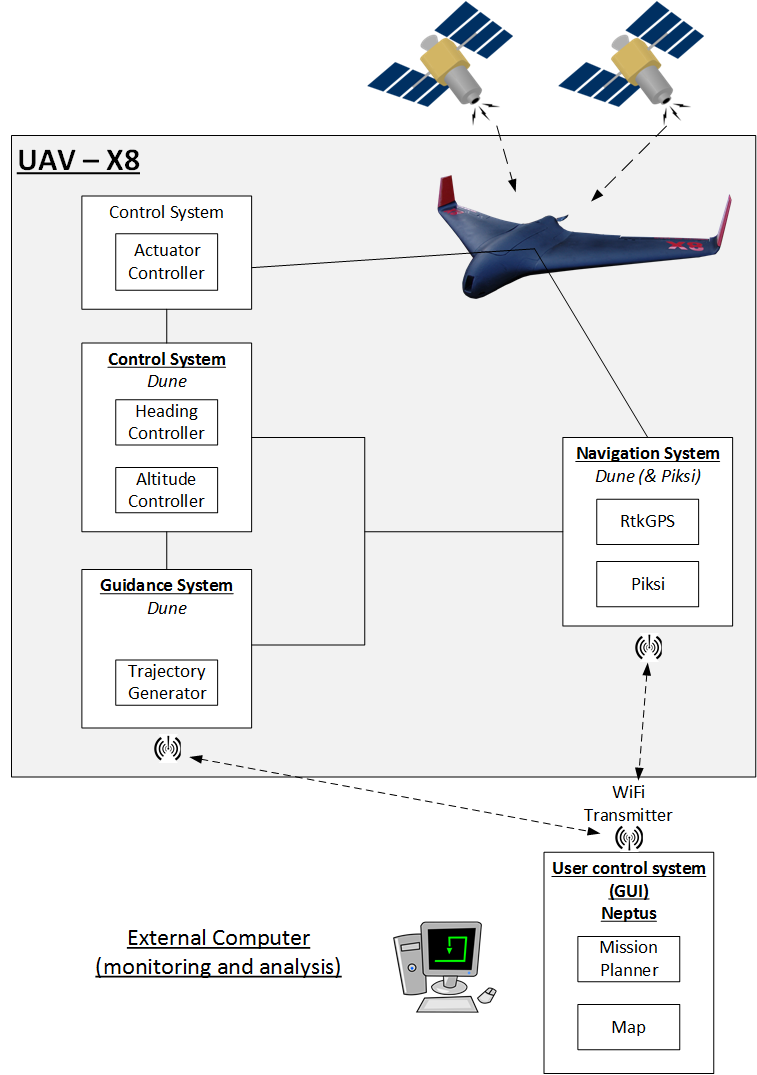
\includegraphics[width=1\textwidth]{figs/System.png}
		\caption{Overview of the automatic net landing system}
		\label{figure:SystemOverview}
\end{figure}

The navigation system apply \gls{rtk-gps} to estimate the relative position of the \gls{uav}. More details of the \gls{rtk-gps} is given in section \ref{ss:rtk-gps}.

The control and guidance system has currently only been tested in \gls{sil} simulations with Ardupilot, which shows promising result likely to be sufficient for automatic landing applications. However this module has not yet been implemented to support the use of \gls{rtk-gps} as required for performing automatic landing.

The \gls{rtk-gps} solution is compute by two different system ,which will be compared against each other, namely Piksi by Swift Navigation and \gls{rtklib} by T. Takasu. The latter is independent on the type of receiver, and thus will be the main focus of this work. More detail about Piksi and Rtklib will be given in \ref{ss:Piksi} and \ref{ss:Rtklib}.

%The comparison test will be used to summarize further work required for complete identification of technology gaps and work required for closure of these gaps such that a control system including provision for automatic landing. This system must be \gls{uav} in a control system. The \gls{uav} that will be used in the test is a Skywalker X8 Fixed Wing \gls{uav}. More details about the X8 will be given in \ref{ss:SkywalkerX8}


%This work will identify and describe the gaps which will need to be closed in order to find a solution which will allow for automatic landing of \glspl{uav}. Two different system that will be compared against each other. 
The current state of the system is that it consist of two parts that has not yet been integrated with each other. The main focus of this project work is the positioning part. The plan is to use \gls{rtk-gps} for positioning estimation. The second part is the guidance and control. Currently there has only been done simulation of the guidance system. It shows promising results, but is yet to be integrated with \gls{rtk-gps}. Figure \ref{figure:SystemOverview} gives a overview of the different modules in the system.

\section{Global Navigation Satellite Systems}
There are currently two operational \gls{gnss} constellations with global coverage, American \gls{gps} and Russian \gls{glonass}. Other \gls{gnss} constellations that will be operational in the near future is the Chinese BeiDou and European Galileo.

The \gls{gps} satellites transmits continuously using two radio frequencies in the L-band referred to as L1 and L2. The L-band covers frequencies between 1 GHz and 2GHz, and is a subset of the ultra high frequency band.

The receiver needs at least four satellite to be able to estimate the receiver position. Three of the satellite is used for the position, and the fourth is used to calculate the receiver clock bias. The position is calculated in the \gls{ecef} reference frame \ref{ss:ECEF}. The geometry of the satellite constellation affect the accuracy of the position estimation. Poor geometry increase the effect of error in the \gls{gps} signal.

There are two basic ways to measure the \gls{gps} signal to estimate a position, which is code and phase measurement. Of the two phase measurment is the most accurate, however also the least reliable due to the integer ambiguities. In code measurement the information in the \gls{gps} signal is used to calculate the psudorange between the receiver and the satellite. The psudorange is the geometric range from the receiver to the satellite in addition to the delay introduce from various error sources. In phase measurement the receiver measures the phase of the \gls{gnss} satellite and compares it against a receiver generated signal. Then by knowing the phase and the frequency function, as well at the start and end epoch time the geometric range between the receiver and satellite can be estimated. It's phase measurement that is mostly used in \gls{rtk-gps}. In phase measurement it's advantageous to know the unknown number of whole cycles between the satellite and the receiver, referred to as integer ambiguity. Estimation of integer ambiguity is called integer ambiguity resolution.

\gls{utc} is standard time on the Earth of which all clock are referred to. \gls{utc} time is defined with the use of atomic clocks, which is also used in \gls{gps}. However the \gls{gps} apply an other time standard namely the \gls{gpst}. The \gls{gpst} is also based on atomic clock in the satellites. Due to the distance from the Earth the \gls{gpst} deviates from the \gls{utc} time. To correct this the \gls{gps} keeps track of the offset between \gls{gpst} and \gls{utc}. The offset is included in the \gls{gps} message as leap seconds to be added to the \gls{gpst}. \gls{gpst} can be given as \gls{tow}, which include the number of weeks since 1980-01-06T00:00Z. \gls{tow} is given in seconds, and is reset each week when the week number is incremented. More information about the \gls{gps} can be found in \citep{GPSBOOK,vik2014integrated} 

\section{Reference frames}
A \gls{gnss} system calculate an estimated position estimated on the Earth where the receiver is. For the position to have any meaning a reference system has to be defined where a frame can be consider as an inertial frame. Based on this a reference frame can be fixed to the Earth rotation, but for local navigation it must be referred to surface of the Earth. This section will present the different reference frame used in global navigation systems.
\subsection{ECI}
\gls{eci} frame is considered a inertial frame for terrestrial navigation. The origin is fixed in the center of the Earth, and the axis is fixed in space. This frame can be considered as an non-accelerating where Newton's laws of motion applies. This is suitable for control system applications as Newtons laws on equation of motion can be used to model the system for control applications.
\subsection{ECEF}\label{ss:ECEF}
The \acrfull{ecef} coordinate system is defined with the origin in the center of the Earth with it's x-axis point toward the intersection between the Greenwich meridian and Equator ( $0\deg $ longitude, $0\deg $ latitude). The z-axis points along the Earth's rotational axis, and the y-axis complete the right handed orthogonal coordinate system. The \gls{ecef} system can be represented in either Cartesian coordinates (xyz) or ellipsoidal coordinates (longitude, latitude and height). The \gls{ecef} frame rotate relative to the \gls{eci} frame at an angular velocity of $\omega_e = 7.2921 \times 10^{-5}rad/s$, where $\omega_e$ is the Earth rotation. Due to the relatively low rotation speed some system can consider the \gls{ecef} frame as inertial, which can simplify the equation of motion for a control system.
\begin{figure}[H]
	\centering
		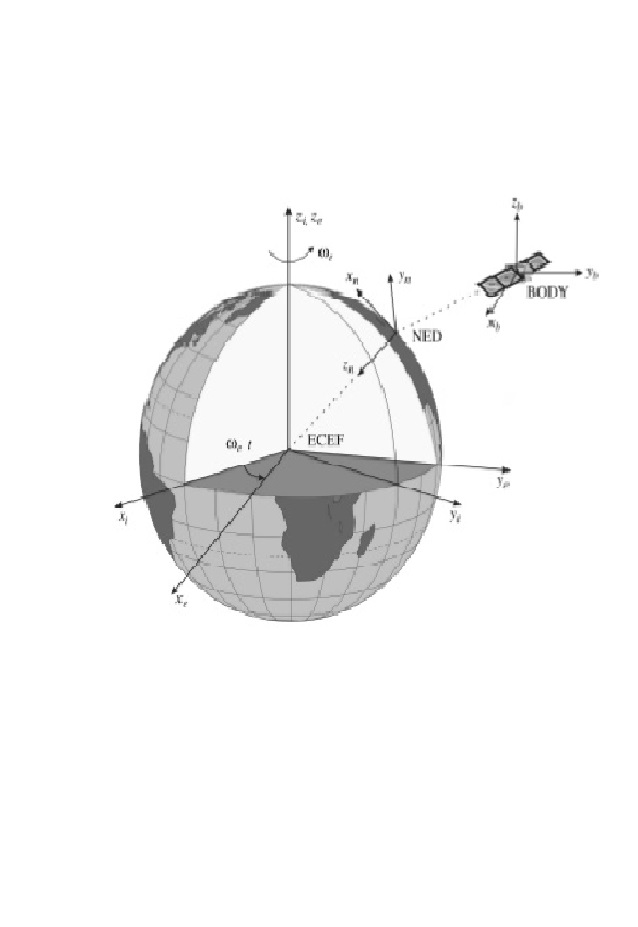
\includegraphics[width=0.7\textwidth]{figs/ECEF-Frame.jpg}
		\caption{The \gls{ecef} frame. Picture from \citep{fossen2011handbook}}
		\label{figure:ECEF}
\end{figure}
\subsection{Local reference frame}
The \gls{ned} and \gls{enu} frame is defined as relative to the Earth reference ellipsoid (\gls{wgs-84}). For the \gls{ned} frame the x axis points in the direction to the true North, y axis towards East while the z axis points downward to completed the right handed orthogonal coordinate system. The \gls{enu} has the x and y axis exchange place with respect to the \gls{ned} frame, and the z axis point upwards instead of downwards.

 
\section{Error sources}
In order to get high accuracy in the position estimation the different error sources must be identified and removed if possible. This section will identify some of the most significant error sources that can affect the \gls{gps} signal, and how to remove or mitigate them in the estimation.
\subsection{Clock error}
There is drift in both the satellite clock and the receiver clock. The atomic clock in the satellites makes the clock drift negligible from the user perspective. The receiver clock tend to drift, and if not taken into account will cause large deviations in the position estimate from the true position. This error is remove by including a fourth satellite in the position computation. The satellite clock error given in the satellite message. 

\subsection{Ionospheric and Trophospheric Delays}
When the \gls{gps} signals travel though the atmosphere there will be a delay caused by the different atmospheric layers.
\subsubsection{Ionospheric delay}
Gas molecules in the ionosphere becomes ionized by the ultraviolet rays that is emitted by the sun, which release free electrons. These electron can influence electromagnetic wave propagation, such as GNSS signals. The delay that the single get from the ionosphere may cause a error the the order of $1-10 meters$. The error can be mitigated by using a double frequency receiver, or by applying a mathematical model to estimate the delay. Both those cases is with a single receiver, however by including a second receiver the GNSS solution system can assume that both receiver receive signal in the same epoch, which means that the signals have experienced the same delay. This will be further explain in \ref{ss: Error mitigation DGPS}.

\subsubsection{Tropospheric delay}
The tropospheric delay is a function of the local temperature, pressure and relative humidity. The delay can vary from $2.4$meters to $25$ meters depending on the elevation angle of the satellites. The error can be mitigated by applying a mathematical model to estimate the tropospheric delay, and by using a elevation mask can remove all satellites with a elevation angle bellow a certain threshold. Error caused by tropospheric delay can be removed in the same manners as ionospheric delay when using two or more receivers. This will be further explain in \ref{ss: Error mitigation DGPS}.

\subsection{Ephemeris Errors}
A satellite is not able to perfectly follow a given orbit, therefore there will be a deviation between satellite position given to the receiver and the true position of the satellite. This is called the ephemeris error. The true position of a satellite is monitored and corrected by the owner of the \gls{gnss} constellation, but error between each correction can be expected.
\subsection{Multipath}
One of the primary source of error in in a GNSS receiver is multipath. Multipath happens when the satellite signal is reflected by a nearby surface before if reach the \gls{gnss} antenna. The delay introduced in the signal can make the receiver believe that its position is several meters away form its true position. The easiest way to mitigated multipath is to place the antenna at a location with open skies, and no tall structures nearby.
%\section{Dilution of Precision}
%The geometry of the \gls{gnss} constellation affect the accuracy of the position solution. Pore geometry will also enhance the effect that different error sources has on the position solution.
\section{Differential GPS}
\acrfull{dgps} consist of at least two receivers, where one is called a base station and the rest rovers. The two receivers are within range of a communication channel over which they are communicating, as shown in figure \ref{figure:DGPS}. The base station has a known position, and the rover estimate the baseline from itself to the base station.

In this project work only phase measurements will be considered for position estimation method.
The problem with precise relative positioning with phase measurement is problem of estimation of integer ambiguities.

\begin{figure}[H]
	\centering
		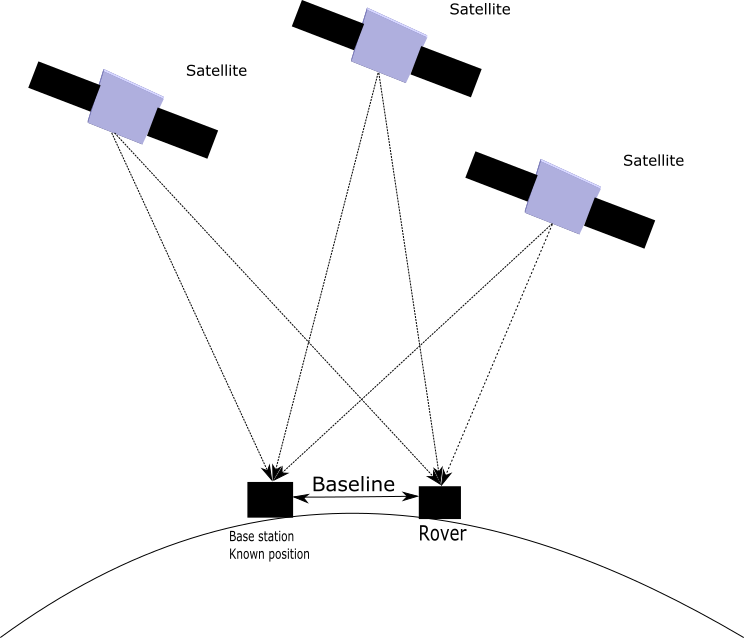
\includegraphics[width=0.7\textwidth]{figs/DGPS.png}
		\caption{Concept figure of \acrfull{dgps}}
		\label{figure:DGPS}
\end{figure}
%\subsection{Integer Ambiguity Resolution Strategy}\label{ss:INtegerAM}
%A well used strategy is the \gls{lambda} method. \gls{lambda} starts by reducing the integer search space by decorrelation adjustment. The \gls{lambda} method has two types of outputs. One is called the fixed solution, and the other is called the float solution. The float solution is the first solution given by the \gls{lambda} method and is used to find the fixed solution. When the right fixed solution is reached the position estimation in from a \gls{dgps} can be considered highly accurate. The solution program can calculate the wrong fixed solution, or experience a cycle slip. In order to reduce the possibility of letting a wrong solution become the fixed solution the program need a integer ambiguity validation strategy. One validation strategy is to check if the ratio between the best ambiguity estimate and the second best estimate in greater then a certain threshold. High \gls{dop} will effect the time the LAMBDA method needs to find a fixed solution.

\subsection{Cycle slip}\label{ss:cycleSlip}
When the integer number of cycles experience a sudden jump in value due to loss of lock of a receiver phase lock it's called cycle slip. The effect of cycle slip is a bias in the measurement large enough to make navigation difficult. The effect of cycle slip will appear as seen in figure \ref{figure:CycleSlip}.
\begin{figure}[H]
	\centering
		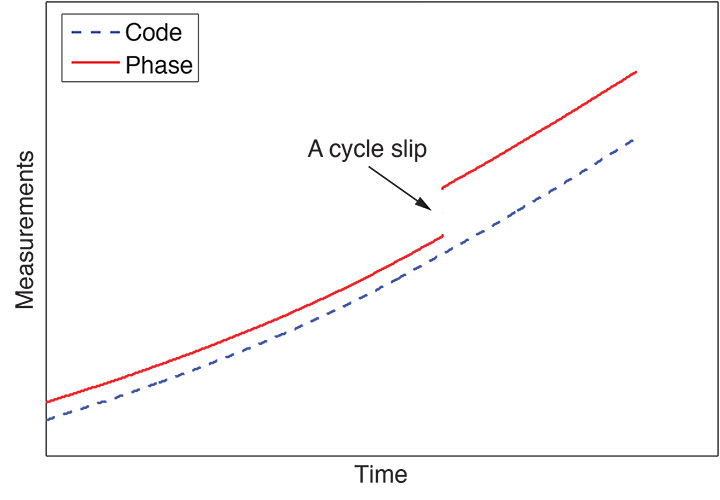
\includegraphics[width=0.7\textwidth]{figs/cycleSlip.jpg}
		\caption{Cycle slip. Picture from \url{http://gpsworld.com/wp-content/uploads/2014/01/I-Fig1.jpg}}
		\label{figure:CycleSlip}
\end{figure}
\subsection{Error mitigation in DGPS} \label{ss: Error mitigation DGPS}
In \gls{dgps} the rover considers that both the rover and base station receive \gls{gps} signal that has experienced the same delay. Thus the rover can remove all error sources that is correlated with the base station. This assumption holds given that the baseline is not to long. For longer baseline other methods must be applied to correct for atmospheric delay. \gls{dgps} error mitigation do not include multipath. Multipath is an uncorrelated error, and thus must be corrected locally by both the rover and base station.


\section{RTK GPS}\label{ss:rtk-gps}
\acrfull{rtk-gps} is a variant of \gls{dgps} system where both the base station and rover receives \gls{gps} signals and the distance between is calculated accurately. The distance between the rover and base station is referred to as a baseline.

\gls{rtk-gps} can either provide a kinematic setting or a moving baseline setting. The difference between the two is that in kinematic the base station has a known stationary position, while in moving baseline the base station position is unknown and allowed to move. The unknown base station is calculated with a single receiver, with the accuracy that entails. Since the base station position is calculated with a single receiver the \gls{rtk-gps} system with moving baseline can never have better global accuracy then what it will get with a single receiver. The advantage with the moving baseline configuration is that \gls{rtk-gps} can be used to find the relative position between two dynamical system using \gls{gnss} in real time. This will be the case in automatic ship landing system, where the base station is on a ship thus must be allowed to move. The advantage with kinematic mode is that it can give a more accurate position estimate. The relative position of the rover can be given in either the \gls{ned} or {enu} frame.

\gls{rtk-gps} systems needs to calculate the position estimate quicker then a standard  system. This is done by sacrificing the correctness of the solution, however in the resent time efficient software and hardware has reduced the this factor.

\cleardoublepage